\mysection{Generación de datos enlazados}
    
    Una vez se han generado los datos de contrataciones mediante el \hyperref[sec:software]{software desarrollado} de acuerdo a las \hyperref[sec:correspondencias]{Correspondencias establecidas entre \texttt{CODICE} y \texttt{OCDS}}, sólo queda el último paso para completar la línea de ejecución: la publicación como \textit{linked data}.

    \begin{figure}[h]
        \centering
        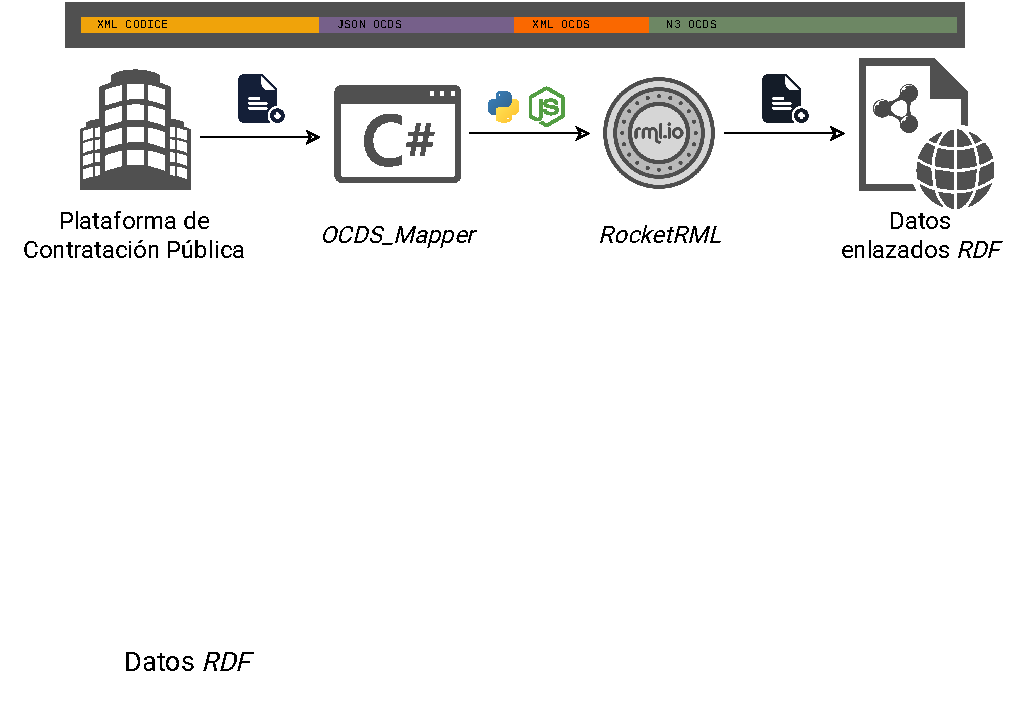
\includegraphics[width=\textwidth]{pipeline.pdf}
        \captionof{figure}{\textit{Pipeline} y formato de los datos en las distintas etapas}
        \label{fig:pipeline}
    \end{figure}
    
    \noindent En la \hyperref[fig:pipeline]{figura 21} se representa el \textit{pipeline} completo, además del formato de los datos a lo largo de las diferentes fases del procesamiento. Los datos de licitaciones originales que provienen de la Plataforma de Contratación Pública están en el formato \texttt{XML} y siguiendo el esquema \texttt{CODICE}. Una vez son procesados por el sistema \textit{OCDS\_Mapper}, éstos pasan al esquema \texttt{OCDS} y al formato \texttt{JSON}. Tras ser mapeados, se transforman mediante un sencillo script en el lenguaje \texttt{Python} (accesible en el repositorio del trabajo \cite{SCRIPTGEN} y en la \hyperref[subsubsec:py1]{sección 10.4.1} del \hyperref[annex:scriptspy]{Anexo IV}) al formato \texttt{XML} para su procesado de reglas \texttt{RML}. Éste se realiza haciendo uso de la librería \textit{RocketRML} \cite{ROCKETRML} (licencia CC-BY-SA 4.0 \cite{LICCC}), ejecutada en el entorno \texttt{Node.js}, para obtener finalmente los datos enlazados \texttt{RDF}.
    \\ \\
    Podría parecer que la transformación a \texttt{JSON} en medio del \textit{pipeline} para posteriormente volver al formato \texttt{XML} inicial es innecesaria, pero esto se hace debido a que \texttt{OCDS} requiere \texttt{JSON} como formato de sus datos, mientras que las reglas de mapeado de \texttt{RML} utilizadas están declaradas haciendo uso de \texttt{XPath}, necesitando \texttt{XML} como formato de entrada.
    
    \subsection{Validación de los datos}
        Previamente a poder realizar la transformación a datos enlazados \texttt{RDF}, es necesario validarlos para poder aseverar la correcta adecuación al estándar \texttt{OCDS} de los mismos. Para ello se ha hecho uso de la herramienta de revisión de \texttt{OCDS} \cite{OCDSREVIEWTOOL} con una batería de múltiples documentos, pero sólo se mostrará el reporte de uno cualquiera en las siguientes figuras.
        
        \begin{figure}[h]
            \centering
            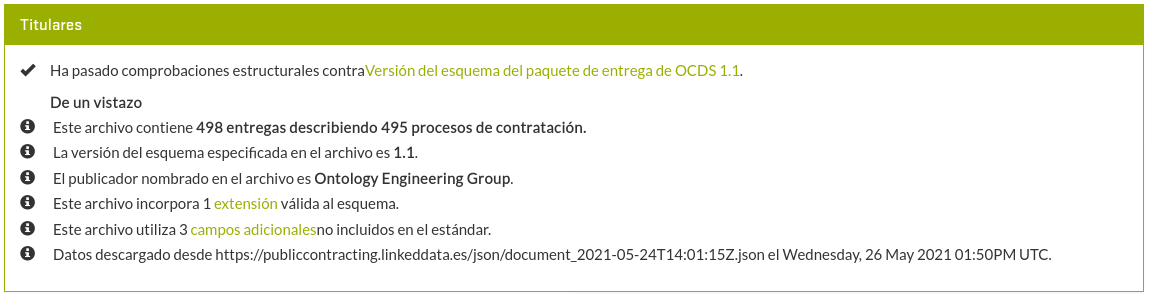
\includegraphics[width=0.925\textwidth]{ocdsreport_1.png}
            \captionof{figure}{Reporte general de la herramienta de revisión de \texttt{OCDS}}
        \end{figure}
        
        \begin{figure}[h]
            \centering
            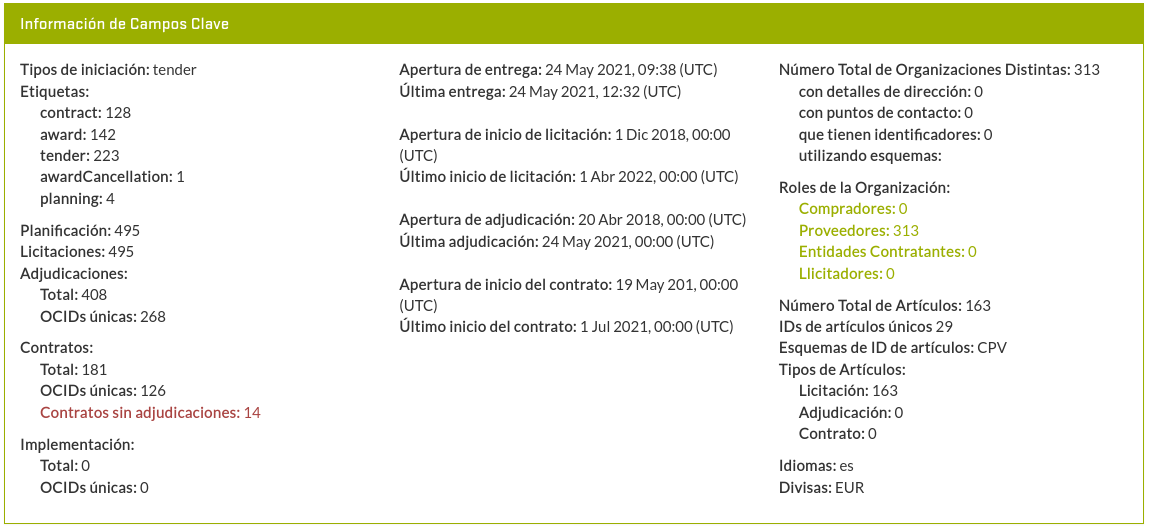
\includegraphics[width=\textwidth]{ocdsreport_2.png}
            \captionof{figure}{Reporte específico de la herramienta de revisión de \texttt{OCDS}}
        \end{figure}
        
        El reporte mostrado como ejemplo es accesible en el siguiente enlace \cite{OCDSREPORT} hasta el día 24 de agosto de 2021, gracias al acceso ofrecido durante 90 días de los reportes ejecutados por la herramienta de revisión.
        
    \subsection{Reglas \texttt{RML}}
        Para poder realizar la transformación a \textit{linked data}, se ha utilizado el lenguaje \texttt{RML} (\texttt{RDF} \textit{Mapping Language}) \cite{RML}, cuyo propósito es mapear información de muy diversas fuentes de información al sistema \texttt{RDF}.
        \\ \\
        Con respecto al procesamiento de las reglas para producir datos \texttt{RDF}, se ha valorado la utilización de dos distintos métodos de ejecución, \textit{RMLMapper} \cite{RMLMAPPER} y \textit{RocketRML} \cite{ROCKETRML}. Sin embargo, debido a la grandísima diferencia de velocidad entre ambas que se puede apreciar en la \hyperref[fig:tiemposrml]{figura 24}, favorable a \textit{RocketRML}, se ha decidido utilizar este software.
        
        \begin{figure}[!htb]
            \centering
            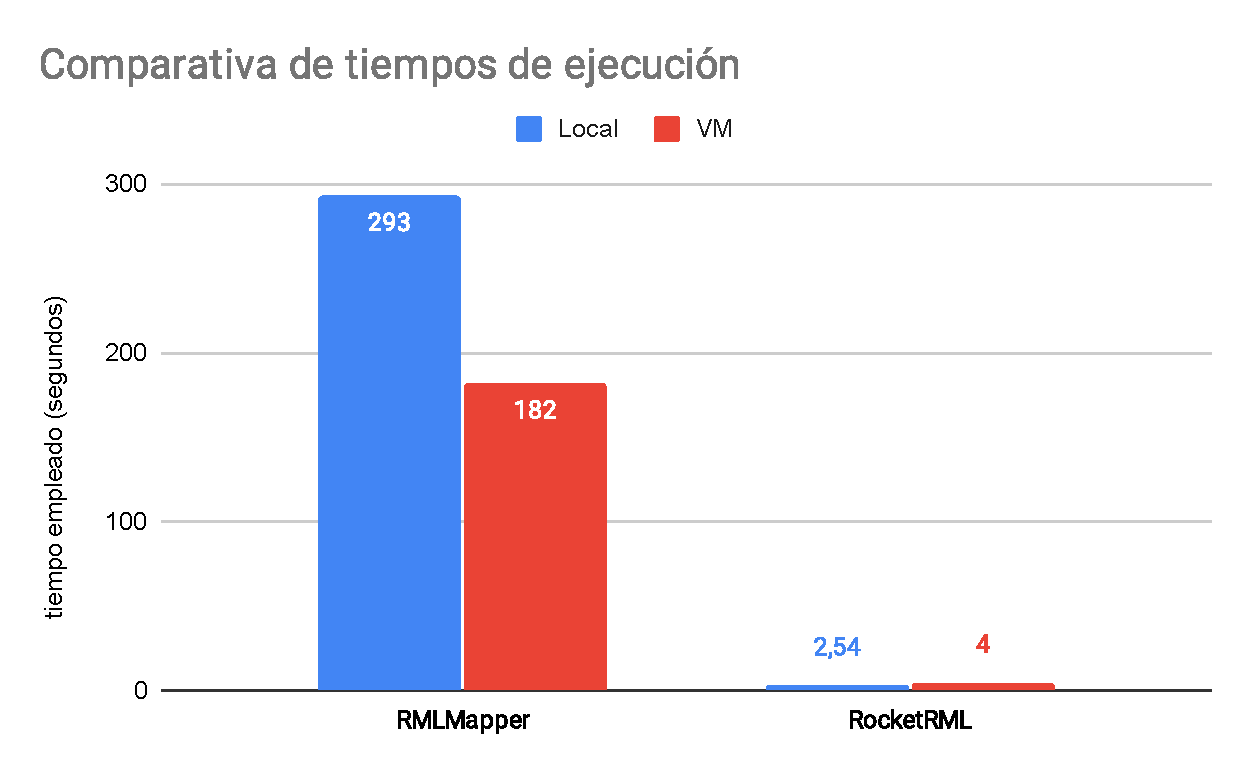
\includegraphics[width=0.7\textwidth]{tiemposrml.pdf}
            \captionof{figure}{Comparativa de tiempos entre \textit{RMLMapper} y \textit{RocketRML}}
            \label{fig:tiemposrml}
        \end{figure}
        
        \noindent Si bien es cierto que la construcción de las reglas se ha ajustado a las necesidades específicas de este proyecto, la mayor parte de éstas son una reutilización de una batería de reglas del proyecto \texttt{TBFY}, accesibles en el siguiente enlace \cite{OPENOPPSMAP}. Sobre ellas se han realizado algunas modificaciones \textit{ad-hoc}, como el cambio de las \texttt{URIs} base (de \texttt{http://data.tbfy.eu} a \texttt{https://publiccontracting.linkeddata.es}), o cambios en algunos \textit{TriplesMap}. Además, se han eliminado aquellas reglas que quedan fuera de las \hyperref[sec:correspondencias]{correspondencias} por motivos de legibilidad de las mismas y agilidad en el procesamiento. El conjunto final de reglas utilizado en el sistema desplegado es accesible en el siguiente enlace del repositorio del trabajo \cite{MYMAP}.
        
    \subsection{Consultas sobre los datos generados} \label{subsec:rdflib}
        Para comprobar que la integridad de los datos enlazados generados se ha preservado tras su procesamiento mediante las reglas \texttt{RML}, se ha confeccionado una batería de consultas \texttt{SPARQL} que asevera que toda la información codificada en dichas reglas se haya preservado.
        \\ \\
        La implementación de las consultas se ha realizado mediante un sencillo script en \texttt{Python} (accesible en el repositorio \cite{SCRIPTRDF} y en la \hyperref[subsubsec:py2]{sección 10.4.2} del \hyperref[annex:scriptspy]{Anexo IV}) haciendo uso de la librería \textit{RDFLib} (licencia BSD 3-Clause \cite{LICBSD3}). El conjunto de \textit{queries} \texttt{SPARQL} se encuentra en el \hyperref[annex:sparql]{Anexo III}.
        \\ \\
        En el repositorio del trabajo se localizan ficheros de ejemplo de la ejecución completa del \textit{pipeline} del sistema, desde los documentos originales \cite{TFGEJ1} hasta los ficheros de texto resultantes de la ejecución de las consultas descritas en esta sección \cite{TFGEJ2}, pasando por su primer procesado a \texttt{JSON} \cite{TFGEJ3} y su versión \texttt{RDF} \cite{TFGEJ4}.
        
    \subsection{Despliegue del sistema}
        Finalmente, el \textit{pipeline} completo, desde la adquisición de documentos de la Plataforma de Contratación Pública hasta la publicación de los datos enlazados ha sido desplegado en una máquina virtual provista para este propósito gracias al \textit{Ontology Engineering Group} \cite{OEG} de la UPM.
        \\ \\
        Dicha máquina virtual está compuesta por 2 procesadores Intel Xeon \texttt{CPU E5-2650 v3 @ 2.30GHz}, con 40 \textit{cores} por procesador. Cuenta asímismo con \texttt{4096 MBs} de memoria \texttt{RAM} de tecnología \texttt{RDIMM} y velocidad \texttt{2133 MT/s}, y su almacenamiento es de \texttt{19 GBs}. El software de virtualización que soporta la infraestructura es \texttt{QEMU-KVM}.
        \\ \\
        En la máquina virtual, mediante el servicio Unix \texttt{cron}, se ha configurado un \textit{script} de ejecución diaria que realiza todas las etapas del procesamiento: en primer lugar, ejecuta el software \textit{OCDS\_Mapper} con el modo de operación \texttt{--daily}, dado que el servicio se ejecuta diariamente, de medianoche, y se pretenden realizar procesamientos de los datos publicados en el día anterior. Una vez se completa esa fase y se realiza el procesado a \texttt{RML} descrito en esta sección, el \textit{script} lleva al directorio \texttt{/var/www/html} dos conjuntos de ficheros: los \texttt{JSON} que devuelve el \textit{OCDS\_Mapper}, de interés por ser documentos válidos con respecto al estándar \texttt{OCDS}, y los correspondientes \texttt{N-Triples} (\texttt{RDF}) que salen de la ejecución del \textit{RocketRML}.
        \\ \\
        Una vez se han colocado los ficheros de interés en los directorios descritos, éstos quedan completamente accesibles a través de la página web \texttt{\url{https://publiccontracting.linkeddata.es}}, para su acceso y consulta.
        
        \begin{figure}[h]
            \centering
            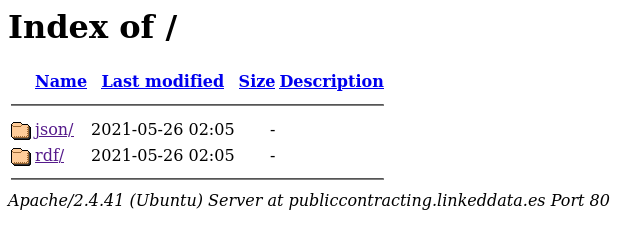
\includegraphics[width=0.755\textwidth]{index.png}
            \captionof{figure}{Captura de la web \texttt{\url{https://publiccontracting.linkeddata.es}}}
        \end{figure}
        
        \begin{figure}[!htb]
            \centering
            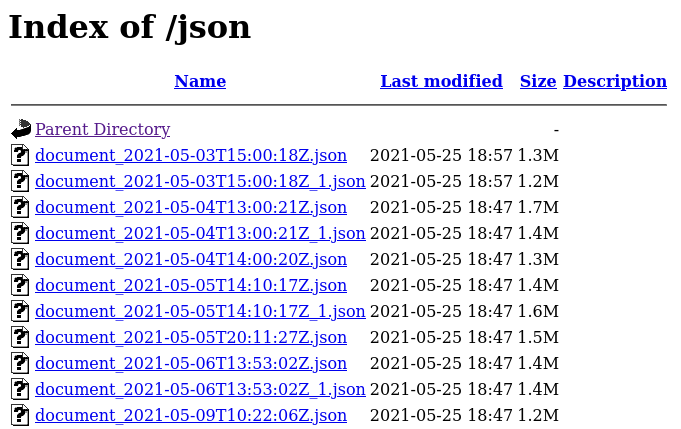
\includegraphics[width=0.755\textwidth]{index_json.png}
            \captionof{figure}{Captura de parte del directorio \texttt{json/} de la web}
        \end{figure}
        
    \vspace{2cm}
    
        \begin{figure}[!htb]
            \centering
            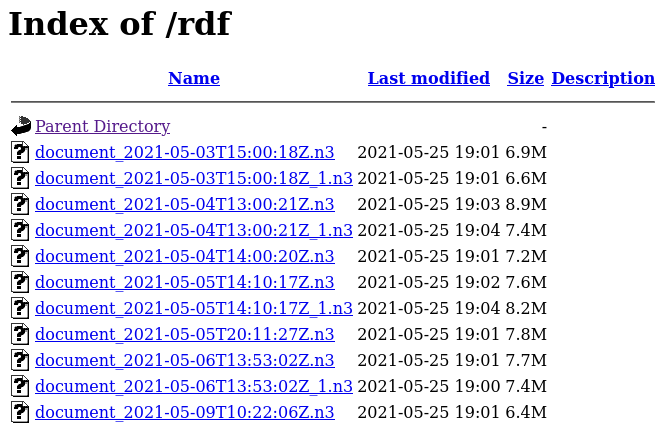
\includegraphics[width=0.755\textwidth]{index_rdf.png}
            \captionof{figure}{Captura de parte del directorio \texttt{rdf/} de la web}
        \end{figure}
    
\newpage